%%%%%%%%%%%%%%%%%%%%%%%%%%%%%%%%%%%%%%%%%%%%%%%%%%%%%%%%%%%%%%%%%%%%%%%%
\chapter{Gas ideali quantistici}
\label{cap:ensquant}
%%%%%%%%%%%%%%%%%%%%%%%%%%%%%%%%%%%%%%%%%%%%%%%%%%%%%%%%%%%%%%%%%%%%%%%%

%%%%%%%%%%%%%%%%%%%%%%%%%%%%%%%%%%%%%%%%%%%%%%%%%%%%%%%%%%%%%%%%%%%%%%%%
\section{Gas ideale nel microcanonico quantistico}
%%%%%%%%%%%%%%%%%%%%%%%%%%%%%%%%%%%%%%%%%%%%%%%%%%%%%%%%%%%%%%%%%%%%%%%%

Prendiamo come al solito un sistema, all'equilibrio termodinamico, formato da $N$ particelle non interagenti e {\em indistinguibili}, racchiuse in un volume $V$ e con un energia totale (fissata) $E$. La terna $(N,V,E)$ rappresenta l'insieme dei parametri microcanonici che definiscono, dal punto di vista termodinamico, il macrostato d'equilibrio del sistema.

La quantità di interesse, quella da cui poi è possibile calcolare tutte le proprietà termodinamiche del sistema {\em via} la sua connessione con l'entropia, è $\Omega(N,V,E)$, cioè il numero di microstati {\em distinti} accessibili al sistema compatibilmente con il macrostato d'equilibrio $(N,V,E)$.

%%%%%%%%%%%%%%%%%%%%%%%%%%%%%%%%%%%%%%%%%%%%%%%%%%%%%%%%%%%%%%%%%%%%%%%%
\subsection{Divisione in celle di energia}
%%%%%%%%%%%%%%%%%%%%%%%%%%%%%%%%%%%%%%%%%%%%%%%%%%%%%%%%%%%%%%%%%%%%%%%%
Come abbiamo già avuto modo di notare parecchie volte in precedenza, in un sistema macroscopico di questo tipo i livelli di energia di {\em singola particella} sono estremamente vicini l'uno all'altro; sembra dunque ragionevole, per semplificare i calcoli, dividere lo spettro energetico del sistema in ``gruppi di livelli'', ovverlo ``celle di energia'' (vedi figura \ref{fig:cellen}).
%%%%%%%%%%%%%%%%%%%%%%%%%%%%%%%%%%%%%%%%%%%%%%%%%%%%%%%%%%%%%%%%%%%%%%%%
\begin{figure}[h!t]
\label{fig:cellen}
\centering
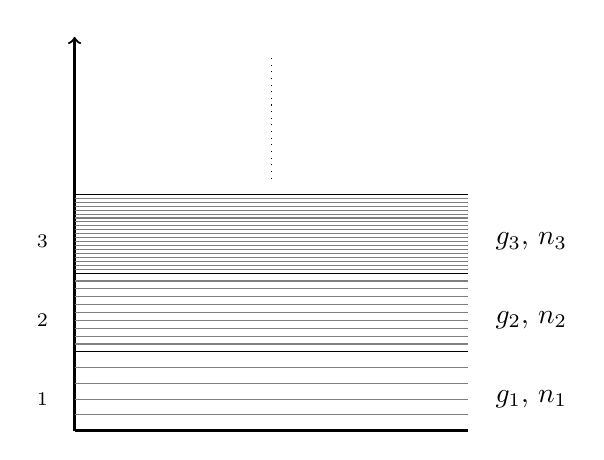
\begin{tikzpicture}
  \draw[thick] (0,0)--(5,0);
  \draw[->,thick] (0,0)--(0,5) node[anchor=east] {$\eps$};  
  \foreach \y in {0.2,0.4,0.6,0.8}
  	\draw[gray] (0,\y)--(5,\y);
  \draw (0,1)--(5,1);
  \draw (-0.4,0.4) node{$\eps_1$};
  \draw (5.8,0.4) node{$g_1$, $n_1$};
  \foreach \y in {1.1,1.2,1.3,1.4,1.5,1.6,1.7,1.8,1.9}
  	\draw[gray] (0,\y)--(5,\y);
  \draw (0,2)--(5,2);
  \draw (-0.4,1.4) node{$\eps_2$};
  \draw (5.8,1.4) node{$g_2$, $n_2$};
  \foreach \y in {2.05,2.1,2.15,2.2,2.25,2.3,2.35,2.4,2.45,2.5,2.55,2.6,2.65,2.7,2.75,2.8,2.85,2.9,2.95}
  	\draw[gray] (0,\y)--(5,\y);
  \draw (0,3)--(5,3);
  \draw (-0.4,2.4) node{$\eps_3$};
  \draw (5.8,2.4) node{$g_3$, $n_3$};
  \draw[dotted] (2.5,3.2)--(2.5,4.8);
\end{tikzpicture}
\caption{Suddivisione (arbitraria) dei livelli energetici di singola particella in celle. La cella $i$--ma ha un'energia media $\eps_i$, ha $g_i$ livelli e contiene $n_i$ particelle.}
\end{figure}
%%%%%%%%%%%%%%%%%%%%%%%%%%%%%%%%%%%%%%%%%%%%%%%%%%%%%%%%%%%%%%%%%%%%%%%%
Sia $\eps_{i}$ l'energia {\em media} della cella $i$-ma e $g_{i}$ il numero (arbitrario) di ``veri'' livelli di energia contenuti nella cella $i$-ma. Supponiamo che la cella contenga $n_{i}$ particelle. Ai fini del nostro calcolo assumiamo che sia $g_{i}$ sia $n_{i}$ siano molto grandi ($g_{i}\gg 1$, $n_{i}\gg 1$). Occorre ricordare e sottolineare che questa divisione in celle di energia è completamente arbitraria, e dunque alla fine dovrà scomparire dal risultato. In particolare il risultato non dovrà dipendere da $g_{i}$, ossia dal modo in cui abbiamo raggruppato i livelli originari del sistema in celle.

Dunque, le $n_{i}$ particelle si disporranno in un certo modo sui $g_{i}$ livelli della cella, e otteniamo una distribuzione $\{n_{i}\}\equiv (n_{0}, n_{1}, n_{2}\dots)$ che dovrà soddisfare i due vincoli seguenti:
\bea
\sum_{i}n_{i} = N \nonumber \\
\sum_{i}n_{i}\eps_{i} = E
\label{eq:vincoliqui}
\eea
Chiamiamo $w(i)$ il numero di microstati {\em distinti} associati alla cella $i-$ma, nella quale $n_{i}$ particelle vengono accomodate su $g_{i}$ livelli; il numero di microstati {\em distinti} dell'intero sistema associati allo specifico set $\nset$ si scrive come
\be
W\nset = \prod_{i}w(i)
\ee
e per definizione abbiamo infine
\be
\Omega(N,V,E) = \sideset{}{'}\sum_{\nset} W\nset
\ee
in cui l'apice sulla somma ricorda che è una somma condizionata dai vincoli dati dalle eq. (\ref{eq:vincoliqui}). Distinguiamo ora i tre casi possibili.

%%%%%%%%%%%%%%%%%%%%%%%%%%%%%%%%%%%%%%%%%%%%%%%%%%%%%%%%%%%%%%%%%%%%%%%%
\subsection{Distribuzione di Bose--Einstein}
%%%%%%%%%%%%%%%%%%%%%%%%%%%%%%%%%%%%%%%%%%%%%%%%%%%%%%%%%%%%%%%%%%%%%%%%
Per trovare $w(i)$ dobbiamo affrontare il problema di sistemare $n_{i}$ oggetti {\em indistinguibili} in $g_{i}$ ``scatole'' {\em distinguibili}. È, a dire la verità, un conto che abbiamo già affrontato: consideriamo $g_{i}+1$ ``stanghette'' (di cui due, quelle agli estremi, fissate: vedi figura \ref{fig:scapal}) e $n_{i}$ ``palline''; il numero richiesto equivale a tutte le permutazioni possibili di $n_{i} + g_{i} - 1$ oggetti, tenendo conto dell'indistinguibilità di palline e stanghette (ma non delle scatole!). Otteniamo quindi facilmente
\be
w_{\textrm{\scriptsize BE}}(i) = \frac{(n_{i} + g_{i} - 1)!}{n_{i}!(g_{i} - 1)!}
\ee
e dunque
\be
W_{\textrm{\scriptsize BE}}\nset = \prod_{i}\frac{(n_{i} + g_{i} - 1)!}{n_{i}!(g_{i} - 1)!}
\ee

%%%%%%%%%%%%%%%%%%%%%%%%%%%%%%%%%%%%%%%%%%%%%%%%%%%%%%%%%%%%%%%%%%%%%%%%
\subsection{Distribuzione di Fermi--Dirac}
%%%%%%%%%%%%%%%%%%%%%%%%%%%%%%%%%%%%%%%%%%%%%%%%%%%%%%%%%%%%%%%%%%%%%%%%
In questo caso, tralasciando il fattore di degenerazione dovuto allo spin, di cui sarà comunque facile tenere conto in seguito, ogni livello può ospitare al massimo una particella, e quindi avremo di necessità $n_{i} \le g_{i}$. Otteniamo quindi $w(i)$ come il numero di modi in cui i $g_{i}$ livelli possono essere divisi in due gruppi: un gruppo costituito da $n_{i}$ livelli occupati e un gruppo formato dai rimanenti $(g_{i}-n_{i})$ livelli occupati:
\be
w_{\textrm{\scriptsize FD}}(i) = \frac{g_{i}!}{n_{i}!(g_{i} - n_{i})!}
\ee
e dunque
\be
W_{\textrm{\scriptsize FD}}\nset = \prod_{i}\frac{g_{i}!}{n_{i}!(g_{i} - n_{i})!}
\ee

%%%%%%%%%%%%%%%%%%%%%%%%%%%%%%%%%%%%%%%%%%%%%%%%%%%%%%%%%%%%%%%%%%%%%%%%
\subsection{Distribuzione di Maxwell--Boltzmann (caso classico)}
%%%%%%%%%%%%%%%%%%%%%%%%%%%%%%%%%%%%%%%%%%%%%%%%%%%%%%%%%%%%%%%%%%%%%%%%
Rideriviamo la statistica di Maxwell--Boltzmann per completezza, anche se è già stata ampiamente trattata. In questo caso le particelle devono in realtà essere considerate come {\em distinguibili}; a causa del fattore correttivo globale di Gibbs convienve considerare direttamente $W_{\textrm{\scriptsize MB}}\nset$. Se consideriamo la singola cella, vediamo che ciascuna delle $n_{i}$ particelle può stare in ognuno dei $g_{i}$ livelli, e tutti gli stati risultati devono essere contati come distinti. Il numero di questi stati è chiaramente pari a $(g_{i})^{n_{i}}$ (è come contare il numero di combinazioni di una schedina del totocalcio: $13$ partite --- ovvero particelle --- che possono stare ognuna, indipendentemente dalle altre, in tre possibili stati: 1, X o 2; il risultato è notoriamente $3^{13}$).

Inoltre il set $\{n_{i}\}$ stesso può essere ottenuto in $N!/(n_{1}! n_{2}!\dots)$ modi diversi, e applicando la correzione di Gibbs otteniamo
\be
W_{\textrm{\scriptsize FD}}\nset = \prod_{i}\frac{(g_{i})^{n_{i}}}{n_{i}!}
\ee

\subsection{Il calcolo dell'entropia}

Calcoliamo l'entropia del sistema:
\be
S(N,V,E) \equiv k\ln\Omega(N,V,E) = k\ln\left[\sideset{}{'}\sum_{\nset}W\nset\right]
\ee
Abbiamo già avuto modo di osservare (vedi sezione \ref{TODO}) %TODO
che il logaritmo della sommatoria, nell'espressione a destra, può essere ben approssimato, nel limite termodinamico, dal logaritmo del termine più grande nella somma. Possiamo dunque scrivere
\be
S(N,V,E) \simeq k\ln W\nsetstar
\ee
in cui $\nsetstar$ è chiaramente il set $(n_1^*,\,n_2^*,\,\ldots\,n_i^*,\,\ldots)$ che massimizza $W$. Gli $n_{i}^{*}$ sono chiaramente i valori {\em più probabili} dei numeri di distribuzione $n_{i}$. $W$ va massimizzato tenendo conto dei vincoli (\ref{eq:vincoliqui}), e quindi usiamo il metodo dei moltiplicatori di Lagrange; inoltre invece di massimizzare $W$ massimizziamo il suo logaritmo, ovvero l'entropia. L'equazione che ci interessa è:
\be
\delta\ln W\{n_{i}\} - \left[ \alpha\sum_{i}\delta n_{i} + \beta\sum_{i}\eps_{i}\delta n_{i}\right] = 0
\label{eq:varlnW}
\ee
Usando l'approssimazione di Stirling otteniamo: \\

\smallskip\noindent
\textsc{Distribuzione di Maxwell--Boltzmann}
\bea
\ln W\nset &=& \ln\prod_{i}\frac{g_{i}^{n_{i}}}{n_{i}!} = \sum_{i}\left[ n_{i}\ln g_{i} -\ln n_{i}!\right]\nonumber \\
&\simeq& \sum_{i}\left[ n_{i}\ln g_{i} -n_{i}\ln n_{i} + n_{i}\right] = 
\sum_{i}\left[ n_{i}\ln(g_{i}/n_{i}) + n_{i}\right]
\eea
\textsc{Distribuzione di Bose--Einstein}
\bea
\ln W\{n_{i}\} &=& \sum_{i}\left[ \ln(n_{i} + g_{i} - 1)! - \ln n_{i}! - \ln(g_{i}-1)!\right] \nonumber\\
&\simeq& \sum_{i}\left[ (n_{i}+g_{i}-1)\ln(n_{i}+g_{i}-1) - n_{i}\ln n_{i} - (g_{i}-1)\ln(g_{i}-1)\right]\nonumber\\
&\simeq& (\mbox{approssimando}\;g_{i}-1\;\mbox{con}\;g_{i})\nonumber\\
&\simeq& \sum_{i}\left[ n_{i}\ln\left(\frac{g_{i}}{n_{i}}+1\right) + g_{i}\ln\left(\frac{n_{i}}{g_{i}}+1\right)\right]
\eea
\textsc{Distribuzione di Fermi--Dirac}
\bea
\ln W\{n_{i}\} &=& \sum_{i}\left[ \ln g_{i}! - \ln n_{i}! - \ln(g_{i}-n_{i})!\right]\nonumber\\
&\simeq& \sum_{i}\left[ g_{i}\ln g_{i} - n_{i}\ln n_{i} - (g_{i}-n_{i})\ln(g_{i}-n_{i})\right]\nonumber\\
&=& \sum_{i}\left[ n_{i}\ln\left(\frac{g_{i}}{n_{i}}-1\right) - g_{i}\ln\left(1-\frac{n_{i}}{g_{i}}\right)\right]
\eea
I tre risultati possono essere condensati in una sola formula introducendo un parametro $a$, in questo modo:
\be
\ln W\nset = \sum_{i}\left[ n_{i}\ln\left(\frac{g_{i}}{n_{i}}-a\right) -\frac{g_{i}}{a}\ln\left(1-a\frac{n_{i}}{g_{i}}\right)\right]
\ee
in cui $a=-1$ rappresenta il caso Bose--Einstein, $a=1$ il caso Fermi--Dirac e il $\lim_{a\to 0}$ il caso Maxwell--Boltzmann.

%%%%%%%%%%%%%%%%%%%%%%%%%%%%%%%%%%%%%%%%%%%%%%%%%%%%%%%%%%%%%%%%%%%%%%%%
\subsection{Il calcolo di $n_{i}^{*}$}
\label{subsec:neps}
%%%%%%%%%%%%%%%%%%%%%%%%%%%%%%%%%%%%%%%%%%%%%%%%%%%%%%%%%%%%%%%%%%%%%%%%

Dobbiamo calcolare la variazione di $\ln W\nset$ per una variazione $\delta\mathbf{n}$. Scriviamo
\be
\delta \ln W\nset = \ln W\{\mathbf{n}+\delta\mathbf{n}\} - \ln W\nset
\ee
e anche, con un leggero abuso di notazione,
\be
\ln W\{\mathbf{n}+\delta\mathbf{n}\} = \ln W\nset + \sum_i \delta n_{i} \dpar{\ln W\nset}{n_{i}} + O((\delta n_{i})^{2})
\ee
Calcolando la derivata
\be
\delta n_{i}\dpar{\ln W\nset}{n_{i}} = \ln\left(\frac{g_{i}}{n_{i}} - a\right) \delta n_{i}
\ee
otteniamo la condizione di massimizzazione
\be
\sum_{i}\left[\ln\left(\frac{g_{i}}{n_{i}} - a\right) -\alpha -\beta\eps_{i}\right]_{n_{i} = n_{i}^{*}}\delta n_{i} = 0
\ee
A questo punto i $\delta n_{i}$ sono arbitrari (non sono più vincolati dall'eq. \ref{eq:vincoliqui}), e perché la somma sia nulla dobbiamo avere che siano nulli separatamente tutti i coefficienti delle variazioni, quindi:
\be
\ln\left(\frac{g_{i}}{n_{i}^{*}} - a\right) -\alpha -\beta\eps_{i} = 0
\ee
da cui si ottiene subito
\be
\frac{n_{i}^{*}}{g_{i}} = \frac{1}{e^{\alpha+\beta\eps_{i}} + a}
\label{eq:nimicro}
\ee
Osserviamo che $n_{i}^{*}/g_{i}$ è il valore più probabile del numero di particelle per livello di energia nella cella $i$-ma: lo reinterpretiamo come il valore più probabile del numero di particelle in un {\em singolo} livello di energia $\eps_{i}$. In questo modo il nostro risultato finale è, come desiderato, indipendente da $g_{i}$, ma va comunque ricordato che, come osservato in precedenza, la procedura di dividere lo spettro d'energia in celle è completamente arbitraria, e sarà dunque meglio ricavare (come faremo in seguito) il risultato (\ref{eq:nimicro}) senza ricorrere a questo espediente.

In ogni caso il risultato che abbiamo appena ottenuto può essere utilizzato per ricavare informazioni importanti, che ci saranno di guida nelle considerazioni che svolgeremo in seguito.

%%%%%%%%%%%%%%%%%%%%%%%%%%%%%%%%%%%%%%%%%%%%%%%%%%%%%%%%%%%%%%%%%%%%%%%%
\subsection{Quantità termodinamiche}.
%%%%%%%%%%%%%%%%%%%%%%%%%%%%%%%%%%%%%%%%%%%%%%%%%%%%%%%%%%%%%%%%%%%%%%%%

Partiamo come al solito dall'entropia, che con un minimo di passaggi algebrici scriviamo in questa forma:
\be
\dfrac{S}{k} \simeq \ln W\nsetstar = \sum_{i}\left[ n_{i}(\alpha + \beta\eps_{i}) + \frac{g_{i}}{a}
\ln\left( 1+ae^{-\alpha-\beta\eps_{i}} \right) \right]
\ee
Poiché $\sum_{i}n_{i}\alpha = \alpha N$ e $\sum_{i}n_{i}\beta\eps_{i} = \beta E$ possiamo scrivere
\be 
\frac{1}{a}\sum_{i}g_{i}\ln\left(1+ae^{-\alpha-\beta\eps_{i}}\right) = \frac{S}{k} - \alpha N -\beta E
\ee
L'interpretazione di $\alpha$ e $\beta$ è la solita, e cioè
\be
\alpha = -\frac{\mu}{kT} 
\quad\quad 
\beta = \frac{1}{kT}
\ee
e possiamo scrivere
\be
\frac{TS + \mu N - E}{kT} = \frac{G - (E-TS)}{kT} = \frac{PV}{kT}
\ee
ottenendo quindi infine
\be
\label{eq:qpot1}
\frac{PV}{kT} = \frac{1}{a}\sum_{i} g_{i}\ln\left( 1+ae^{(\mu-\eps_{i})/kT} \right)
\ee
Nel caso della statistica di Maxwell--Boltzmann ricaviamo immediatamente, mandando $a\to 0$, l'equazione di stato dei gas perfetti:
\be
PV = kT\sum_{i}g_{i}e^{-\alpha-\beta\eps_{i}} = kT\sum_{i}n_{i}^{*} = NkT
\ee
Notiamo che il termine a destra della (\ref{eq:qpot1}), essendo uguale a $PV/kT$, deve corrispondere al $q$--potenziale del sistema. Prima di fare questa identificazione sarà meglio svolgere il conto nel grancanonico per eliminare dal discorso l'arbitraria suddivisione dell'energia in celle.

%%%%%%%%%%%%%%%%%%%%%%%%%%%%%%%%%%%%%%%%%%%%%%%%%%%%%%%%%%%%%%%%%%%%%%%%
\section{Gas ideali quantistici nel canonico e nel grancanonico}
%%%%%%%%%%%%%%%%%%%%%%%%%%%%%%%%%%%%%%%%%%%%%%%%%%%%%%%%%%%%%%%%%%%%%%%%

Tenendo conto dei conti quantistici che abbiamo svolto nel capitolo precedente, possiamo scrivere la funzione di partizione canonica di un gas ideale in questo modo:
\be
\label{eq:partcanq}
Q_N(V,T) = \sideset{}{'}\sum_{\nset} g\nset e^{-\beta\sum_\eps n_\eps\eps}
\ee
in cui $n_\eps$ è il numero di particelle nel livello di energia di singola particella $\eps$; dovranno ovviamente valere le seguenti relazioni:
\bea
\label{eq:vicanq}
\sum_\eps n_\eps &=& N\nonumber\\
\sum_\eps n_\eps\eps &=& E
\eea
L'apice sulla somma in (\ref{eq:partcanq}) ci ricorda che non possiamo sommare su tutti i set di distribuzione $\nset$ ma solo su quelli che soddisfano il vincolo espresso dalla prima delle (\ref{eq:vicanq}), perché nel canonico il numero di particelle $N$ è fissato. Il fattore di peso statistico $g\nset$ cambia a seconda della statistica che usiamo. Nel caso di Maxwell--Boltzmann abbiamo
\be
\label{eq:gqMB}
g_{\text{MB}}\nset = \dfrac{1}{\prod_\eps n_\eps!}
\ee
nel caso di Bose--Einstein abbiamo
\be
g_{\text{BE}}\nset = 1
\ee
e infine nel caso di Fermi--Dirac abbiamo
\be
g_{\text{FD}}\nset = \left\{
\begin{array}{ll}
1 & \text{se tutti gli\ } n_\eps = 0 \text{\ o\ } $1$ \\
0 & \text{altrimenti}
\end{array} \right.
\ee
Va notato che ora stiamo lavorando con gli stati di singola particella come veri stati individuali, senza richiedere il raggruppamento nelle celle d'energia che abbiamo introdotto in precedenza.

Prima di tutto recuperiamo un risultato noto, ossia la funzione di partizione canonica nel caso di Maxwell--Boltzmann. Moltiplicando per $1 = N!/N!$ possiamo scrivere
\be
Q_N(V,T) = \dfrac{1}{N!}\sideset{}{'}\sum_{\nset}\left[
\dfrac{N!}{\prod_\eps n_\eps!}\prod_\eps\left(
e^{-\beta\eps}
\right)^{n_\eps}
\right]
\ee
Ma ora proprio a causa del vincolo (\ref{eq:vicanq}) possiamo usare il teorema multinomiale e scrivere
\be
Q_N(V,T) = \dfrac{1}{N!}\left[
\sum_\eps e^{-\beta\eps}
\right]^N = \dfrac{1}{N!}[Q_1(V,T)]^N = \dfrac{1}{N!}\left(\dfrac{V}{\lambda^3}\right)^N
\ee
È rassicurante osservare come il formalismo quantistico applicato alla statistica di Maxwell--Boltzmann abbia riprodotto il ben noto caso classico.

Nel caso dei gas quantistici propriamente detti, invece, il teorema multinomiale non è di nessun aiuto, e il vincolo cui è sottoposta la sommatoria che definisce la funzione di partizione canonica rende il calcolo molto complicato. Passiamo quindi direttamente al formalismo grancanonico, in cui, sorprendentemente, il calcolo risulta invece molto semplice. Scriviamo la funzione di partizione grancanonica:
\bea
\calQ(z,V,T) &=& \sum_{N=0}^{\infty}\left[
z^N \sideset{}{'}\sum_{\nset} e^{-\beta\sum_\eps n_\eps\eps}
\right] \nonumber\\
&=& \sum_{N=0}^{\infty}\left[
\sideset{}{'}\sum_{\nset}\prod_\eps\left(
ze^{-\beta\eps}
\right)^{n_\eps}
\right]
\eea
Ma ora la doppia sommatoria nell'equazione che precede, la prima su tutti i possibili valori di $N$ e la seconda, vincolata, sui possibili set $\nset$, ha il miracoloso effetto di far sparire il vincolo: possiamo quindi sommare su tutti gli $n_\eps$ {\em indipendentemente} l'uno dall'altro, e questo ci semplifica notevolmente la vita. Possiamo dunque scrivere
\bea
\calQ(z,V,T) &=& \sum_{n_0,\,n_1,\,\ldots} \left[
\left( ze^{-\beta\eps_0}\right)^{n_0}
\left( ze^{-\beta\eps_1}\right)^{n_1}\cdots
\right]\nonumber\\
&=& 
\left[\sum_{n_0}\left( ze^{-\beta\eps_0}\right)^{n_0}\right]
\left[\sum_{n_1}\left( ze^{-\beta\eps_1}\right)^{n_1}\right]\cdots
\eea
Nel caso di Bose--Einstein gli $n_\eps$ possono assumere qualsiasi valore da $0$ a $\infty$. Se poniamo la condizione $z\exp(-\beta\eps) < 1$ per ogni $\eps$ possiamo risommare le serie geometriche e scrivere
\be
\calQ_{\text{BE}}(z,V,T) = \prod_\eps\dfrac{1}{1-ze^{-\beta\eps}}
\ee
Nel caso di Fermi--Dirac invece, $n_\eps = 0, 1$. Otteniamo dunque immediatamente
\be
\calQ_{\text{FD}}(z,V,T) = \prod_\eps \left( 1+ze^{-\beta\eps} \right)
\ee
Dallo studio del grancanonico nel caso classico sappiamo che possiamo scrivere, per il $q$--potenziale,
\be
q(z,V,T) = \dfrac{PV}{kT} = \ln \calQ(z,V,T) = \mp \sum_\eps \ln\left(
1 \mp z e^{-\beta\eps}
\right)
\ee
in cui il segno negativo vale per i bosoni mentre il segno positivo vale per i fermioni.

Reintroducendo il parametro $a$ possiamo scrivere, per tutte e tre le statistiche,
\be
q(z,V,T) = \dfrac{PV}{kT} =  \dfrac{1}{a} \sum_\eps \ln\left(
1 + a z e^{-\beta\eps}
\right)
\ee
e ricordiamo che il limite $a\to 0$ vale nel caso MB, il caso $a=-1$ vale per $BE$ e il caso $a=1$ vale per $FD$. È facile vedere che nel limite $a\to 0$ ritroviamo il noto risultato classico
\be
q_{\text{MB}} = z\sum_\eps e^{-\beta\eps} = z\,Q_1
\ee
Applicando le formule valide per l'\ensemble\ grancanonico possiamo scrivere
\bea
N &=& z\dparc{q}{z}{V,T} = \sum_\eps \dfrac{1}{z^{-1}e^{\beta\eps} + a}\nonumber\\
U &=& -\dparc{q}{\beta}{z,V} = \sum_\eps \dfrac{\eps}{z^{-1}e^{\beta\eps} + a}
\eea
Osservando le equazioni precedenti sembra logico concludere che il valore d'aspettazione $\langle n_\eps\rangle$ per il numero medio di particelle sul livello $\eps$ sia pari a
\be
\langle n_\eps\rangle = \dfrac{1}{z^{-1}e^{\beta\eps} + a}
\ee
Questo può essere controllato con un conto esplicito:
\be
\label{eq:numocceps}
\langle n_\eps\rangle = -\dfrac{1}{\beta}\dparc{q}{\eps}{z,T,\;\text{tutte le altre\ }\eps} = \dfrac{1}{z^{-1}e^{\beta\eps} + a}
\ee
Troviamo quindi un risultato che avevamo anticipato, ossia che il valore medio $\langle n_\eps\rangle$ è uguale al valore più probabile $n_\eps^*$.

%%%%%%%%%%%%%%%%%%%%%%%%%%%%%%%%%%%%%%%%%%%%%%%%%%%%%%%%%%%%%%%%%%%%%%%%
\section{Statistica dei numeri d'occupazione}
%%%%%%%%%%%%%%%%%%%%%%%%%%%%%%%%%%%%%%%%%%%%%%%%%%%%%%%%%%%%%%%%%%%%%%%%

L'equazione (\ref{eq:numocceps}) ci fornisce il numero medio d'occupazione di un livello d'energia $\eps$ di singola particella come funzione esplicita della quantità $(\eps-\mu)/kT$, in cui $\mu$ è evidentemente il potenziale chimico del sistema:
\be
\langle n_\eps\rangle = \dfrac{1}{e^{(\eps-\mu)/kT} + a}
\ee
L'andamento funzionale di questa quantità, per le tre diverse statistiche, è mostrato in figura \ref{fig:numocc}.
%%%%%%%%%%%%%%%%%%%%%%%%%%%%%%%%%%%%%%%%%%%%%%%%%%%%%%%%%%%%%%%%%%%%%%%%
\begin{figure}[h!t]
  \centering
\begin{tikzpicture}[domain={-2.2:2.2},xscale=2.5,yscale=3]
  \draw[->] (0,0) -- (0,2) node[anchor=east] {$\langle n_\eps\rangle$};
  \foreach \y in {1}
    \draw (1pt,\y cm) -- (-1pt,\y cm) node[anchor=east] {$\y$};
  \draw[->] (-2.2,0) -- (2.2,0) node[anchor=north] {$(\eps-\mu)/kT$};
  \draw[dotted,gray] (-2.2,1)--(2.2,1);
  \draw plot[id=numocc1,domain={-0.5:2.1}] function{exp(-x)};
  \draw plot[id=numocc2,domain={0.5:2.1}] function{1/(exp(x)-1)};
  \draw plot[id=numocc3,domain={-2.1:2.1}] function{1/(exp(x)+1)};
  \draw (-1.8,0.7) node{FD};
  \draw (-0.7,1.5) node{MB};
  \draw (0.8,1.5)  node{BE};

\end{tikzpicture}
  \caption{Il numero d'occupazione medio $\langle n_\eps\rangle$ per le tre statistiche.} 
  \label{fig:numocc}
\end{figure}
%%%%%%%%%%%%%%%%%%%%%%%%%%%%%%%%%%%%%%%%%%%%%%%%%%%%%%%%%%%%%%%%%%%%%%%%
È necessario notare alcuni fatti. Prima di tutto, osserviamo che le due curve ``quantistiche'' convergono alla curva classica (MB) per grandi valori di $(\eps-\mu)/kT$. In questo limite vediamo anche che il valore di $\langle n_\eps\rangle$ va esponenzialmente a zero. Dunque il fattore statistico classico $g_{\text{MB}}{\nset}$, vedi eq. (\ref{eq:gqMB}), tende molto velocemente a $1$; la distinzione tra trattamento classico e trattamento quantistico diventa insignificante. Siamo però costretti a osservare che il limite classico lo si raggiunge per alte temperature. Ciò implica che in questo limite il potenziale chimico $\mu$ deve essere negativo e molto grande in valore assoluto; proprio perché, {\em per qualsiasi valore di} $\eps$, la quantità $(\eps-\mu)/kT$ sta andando all'infinito (positivo) mentre anche la stessa $T$, che sta al denominatore, va all'infinito. Dunque in questo limite la fugacità $z = \exp(\mu/kT)$ tende a $0$. Per un gas ideale classico abbiamo
\be
q(z,V,T) = \dfrac{PV}{kT} = \dfrac{zV}{\lambda^3}
\ee
e utilizzando l'equazione di stato $P/kT = N/V = n$ otteniamo
\be
z = n\lambda^3
\ee
Dunque il fatto che $z$ diventi molto piccola nel limite classico, per tutte le statistiche, esprime di nuovo la condizione di {\em classicità} che abbiamo già ricavato:
\be
n\lambda^3 \ll 1
\ee
Per terminare la discussione sul caso classico notiamo che sebbene abbiamo disegnato la curva (MB) anche per valori piccoli e addirittura negativi dell'ordinata, la curva stessa ha senso solo nella parte destra del grafico. Infatti non appena $\langle n_\eps\rangle$ diventa sostanzialmente diverso da zero l'approssimazione classica smette di avere alcun senso.

Nel caso (BE) notiamo che deve valere la condizione $ze^{-\beta\eps} < 1$ per ogni valore di $\eps$. In particolare dovrà valere per lo stato di minima energia, $\eps = 0$. Quindi per un gas di BE avremo sempre $z < 1$, cioè $\mu < 0$. Come vedremo meglio nel prossimo capitolo, nel limite in cui $z\to 1$ compare un fenomeno fisico molto interessante, la così detta {\em condensazione di Bose--Einstein}.

Nel gas di (FD) invece il valore di $z$ non ha nessun limite; partendo da $0$ può crescere indefinitamente. Questo significa che $\mu$ può diventare positivo. Anche in questo caso vedremo che esiste un limite, quello in cui $T\to 0$ e $\mu \to\mu_0$, che ha delle profondissime implicazioni fisiche (gas degenere di Fermi).

%%%%%%%%%%%%%%%%%%%%%%%%%%%%%%%%%%%%%%%%%%%%%%%%%%%%%%%%%%%%%%%%%%%%%%%%
\section{Rivisitazione delle considerazioni cinetiche}
%%%%%%%%%%%%%%%%%%%%%%%%%%%%%%%%%%%%%%%%%%%%%%%%%%%%%%%%%%%%%%%%%%%%%%%%
Nel capitolo \ref{cap:complementi}, e in particolare nella sezione \ref{sec:conskin}, abbiamo svolto alcune considerazioni cinetiche, in particolare sulla pressione di un gas ideale e sulla sua effusione, utilizzando la statistica di Maxwell--Boltzmann. In questa sezione ci occuperemo delle stesse questioni, ma usando la statistica generalizzata valida anche per i casi quantistici.

Abbiamo visto che possiamo scrivere
\be
N = \sum_\eps \langle n_\eps \rangle
\ee
L'energia $\eps$ è in tutta generalità una funzione del momento $p$; passando dunque all'integrale e usando la densità degli stati $g(p)$ possiamo scrivere
\be
\label{eq:nconskin2}
\dfrac{N}{V} = \dfrac{4\pi}{h^3}\int_0^\infty \dfrac{p^2}{z^{-1}e^{\eps(p)}-1}
\ee
Passiamo alla pressione: possiamo scrivere
\bea
\label{eq:pconskin21}
PV &=& \dfrac{kT}{a}\sum_\eps \log\left(
1 + aze^{-\beta\eps(p)}
\right) \nonumber\\
&=& \dfrac{4\pi VkT}{a h^3}\int_0^\infty \de{p}\,p^2\,\log\left(
1 + aze^{-\beta\eps(p)}
\right)
\eea
in cui siamo ancora una volta passati all'integrale usando la densità degli stati. Integrando per parti otteniamo
\bea
\label{eq:pconskin22}
P &=& \dfrac{4\pi kT}{ah^3} \left\{
\left[
\dfrac{p^3}{3} \log\left(1 + aze^{-\beta\eps(p)}\right)
\right]_0^\infty \right. \nonumber \\
&+& \left. \int_0^\infty \dfrac{p^3}{3}\dfrac{aze^{-\beta\eps(p)}}{1+aze^{-\beta\eps(p)}}
\, \beta \, \dfrac{\de{\eps}}{\de{p}}\,\de{p}
\right\} \nonumber \\
&=& \dfrac{4\pi}{3h^3}\int_0^\infty \de{p}\, p^2 \dfrac{1}{z^{-1}e^{\beta\eps(p)}}
\left( p\dfrac{\de{\eps}}{\de{p}} \right)
\eea
risultato ottenuto considerando che la parentesi quadra svanisce a entrambi i limiti d'integrazione. Confrontando la (\ref{eq:pconskin22}) con la (\ref{eq:nconskin2}) otteniamo
\be
\label{eq:pkinognistat}
P = \dfrac{n}{3}\left\langle p\dfrac{\de{\eps}}{\de{p}}\right\rangle 
= \dfrac{n}{3}\langle pv \rangle
\ee
Notiamo che questo risultato vale qualunque sia la statistica utilizzata. Notiamo anche che se $\eps$ è della forma $\eps \propto p^s$ abbiamo
\be
p\dfrac{\de{\eps}}{\de{p}} = s\eps
\ee
e dunque
\be
P = \dfrac{s}{3}n\langle \eps \rangle = \dfrac{sU}{3V}
\ee
Non si tarda a riconoscere il caso $s=1$, cioè $\eps = cp$ (caso ultrarelativistico), e quello $\eps = p^2/2m$ (caso non relativistico). Anche quest'ultima equazione è valida qualunque sia la statistica usata.

\begin{Exercise}
Usando la (\ref{eq:pkinognistat}) recuperare, usando la statistica di MB, l'equazione di stato dei gas ideali classici.
\end{Exercise}

\noindent
Per calcolare il {\em rate} di effusione per unità di area, dobbiamo calcolare quante molecole, nell'unità di tempo, colpiscono una determinata parete del contenitore (diciamo quella perpendicolare all'asse $z$, verso l'alto) e poi dividere per l'area stessa della parete. Ripeteremo con poche variazioni i ragionamenti fatti nella sottosezione \ref{subsec:effusione}. Qualunque sia la statistica utilizzata, chiamiamo $f(\myvec{v})$ la distribuzione in velocità delle molecole del gas, considerandola normalizzata:
\be
4\pi\int_0^\infty \de{v}\,v^2\,f(v) = 1
\ee
Il numero totale di particelle che nell'intervallo di tempo $\de{t}$ colpiscono un'area unitaria della parete di cui sopra sarà dato (vedi sottosezione \ref{subsec:effusione}) da
\bea
\label{eq:effgen}
R &=& n \iint_{-\infty}^{\infty}\de{v_x} \, \de{v_y}\int_0^\infty \de{v_z} \, v_z \,
f(\myvec{v}) \nonumber \\
&=& \int_0^{2\pi}\de{\phi}\int_0^{\pi/2}\de{\theta}\int_0^{\infty}
v \cos\theta \, f(v) \, v^2\de{v} \, \sin\theta \, \de{\theta} \, \de{\phi}
\nonumber \\
&=& \pi n\int_0^\infty \de{v} \, v^3 \, f(v) = \dfrac{n}{4}\langle v \rangle
\eea
Anche questo risultato, identico a quello ottenuto nella sottosezione \ref{subsec:effusione}, è indipendente dalla statistica usata, e continua a valere anche nel caso ultrarelativistico; come vedremo ciò sarà importante nello studio della raziazione di corpo nero.